\documentclass[]{article}
\usepackage{graphicx}
\usepackage{subcaption}
\usepackage{siunitx}
\usepackage{longtable}
\usepackage{tabu}
\usepackage{booktabs}
%opening
\title{Reply to NST reviewers}
\author{Zhou Yong}

\begin{document}

\maketitle

\section{Reviewer 1}
\subsection{Question: Why not show $G_{relative}$ distribution against the reference PMT}
\textit{Original statements: P.7 - Fig.7: I believe it would be preferable to show th plot of $G_{relative}$ with respect one of the reference PMT, which remain untouched during the full set of measurements (if I understand well the procedure).} \newline
\textbf{Answer:}
\begin{enumerate}
	\item Although the two fixed PMTs can be used to calculate the $G_{relative}$ of all tested PMTs, they are not necessarily to be adopted as reference PMTs.  Acctually, they are called monitoring PMT  in our test bench system. As pointed out in the general description of the test bench in Sec. 2 of the article, these two PMTs are mainly used to monitor the LED stability and overall performance of the test bench system. 
	\item Since a relative method is adopted, any one PMT can be used to get a specific $G_{relative}$ distribution. In other words, the $G_{relative}$ is dependent on the selection of reference PMT. The selection of reference PMT is mainly determined by the purpose of the test bench user. In PSD PMT characterization, the reference  PMT is the one which has been coupled to a prototype detector unit and then underwent a cosmic ray calibration. The optimal working voltage of the reference PMT has been determined through the cosmic ray calibration. Since we can calculate $G_relative$ of all other PMTs with respect to this reference PMT and its variation against supplying voltage, the optimal working voltages for all PMTs can be determined in this way.  
	\item The above procedure for  PSD PMT voltage adjustment is not the subject of this article, thus not described in the article. In this article, the PMT with the smallest gain has been chosen as the reference PMT to calculate the $G_{relative}$ because this gives the reader a clear implication of the variation of the gain of the R4443 tubes.
\end{enumerate}

\subsection{Question: More detalis about the integrating sphere and how it works as a perfect integrator for short light pulses}
\textit{Original statements: P.4 - L.36: Can you provide some more details on the integrating sphere and in particular how it works as a perfect light integrator even for relatively short duration pulse of the order of few tens of ns?}\newline
\textbf{Answer:} \newline
baffle
coating material
multiple scattering reflection
diffuse white reflective coating
\begin{figure}
	\centering
	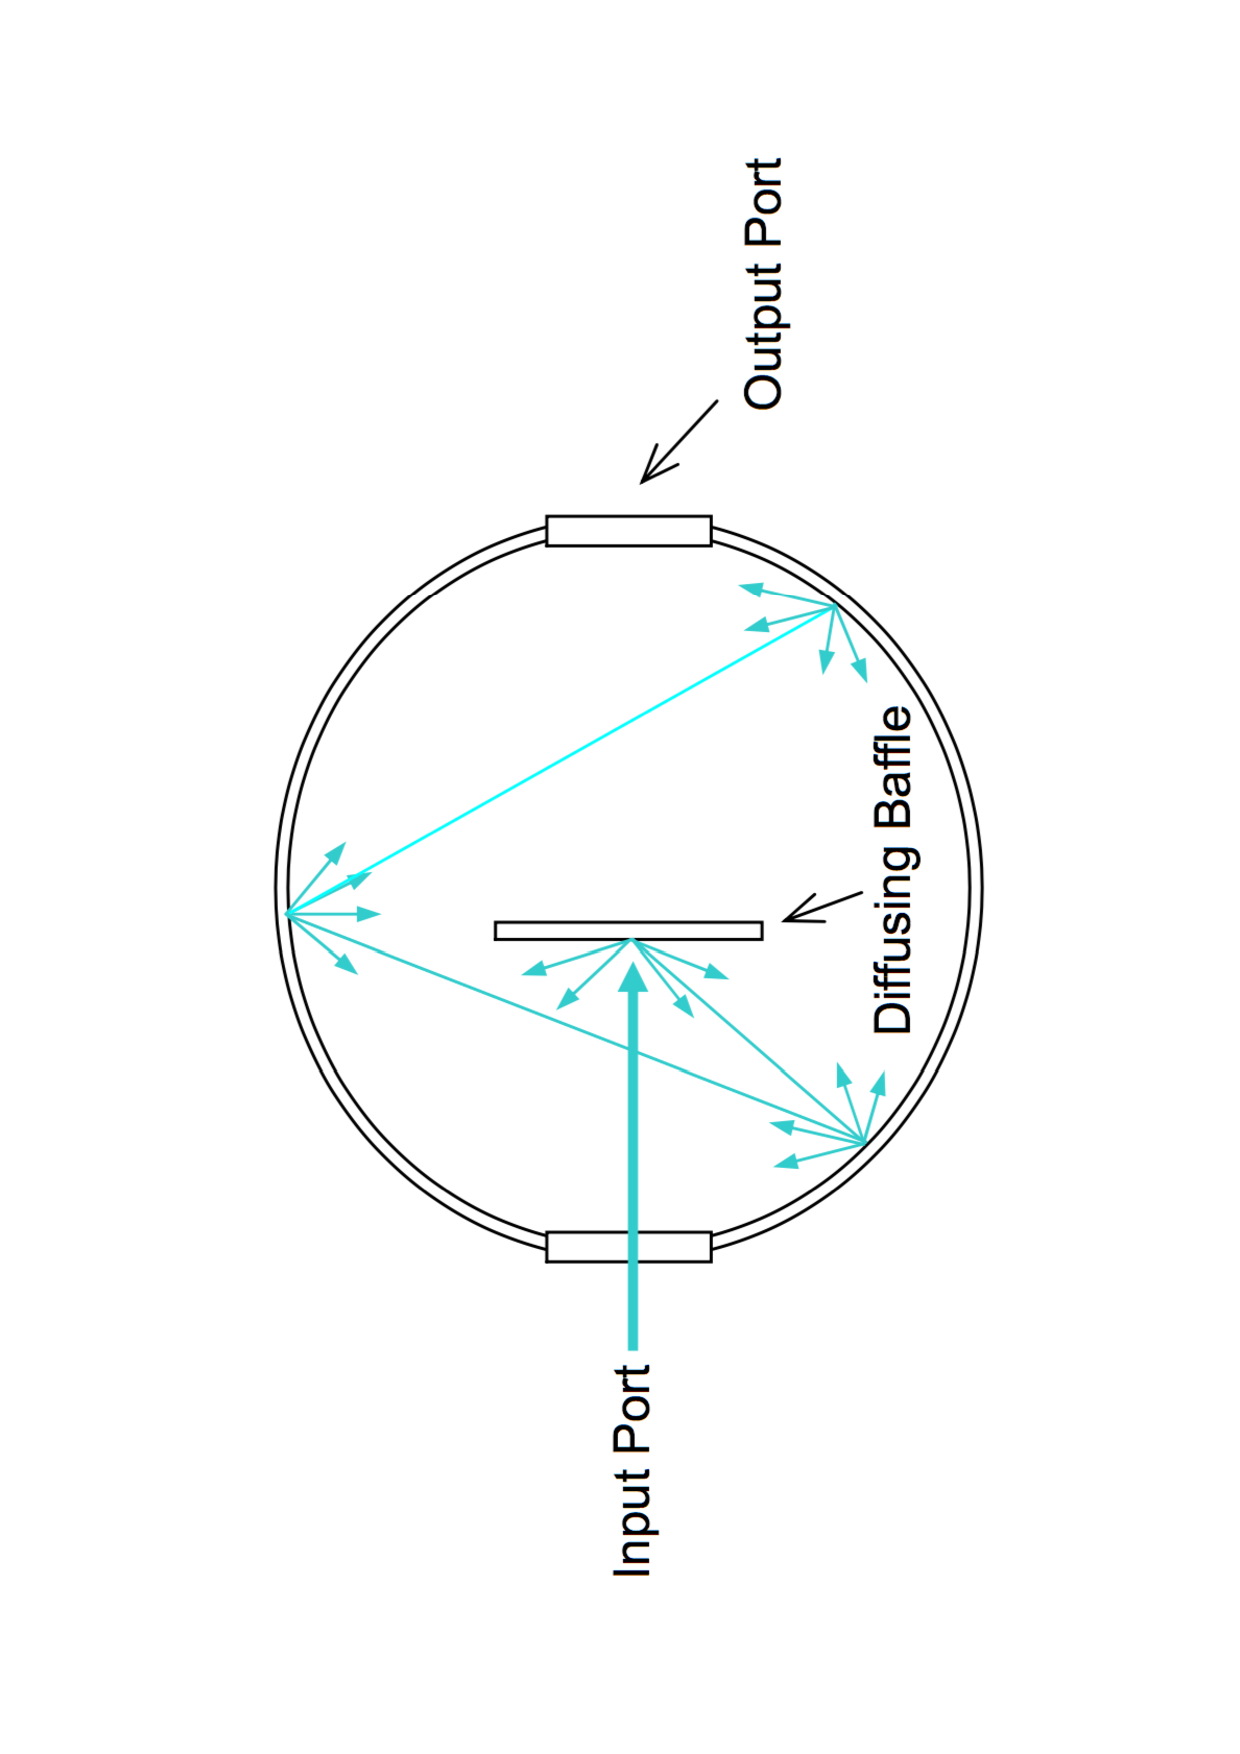
\includegraphics[width=0.8\textwidth,angle=-90]{is_principle}
	\caption{Integrating Sphere working principle}
\end{figure}

\begin{figure}[!htb]
	\begin{subfigure}[t]{75mm}
		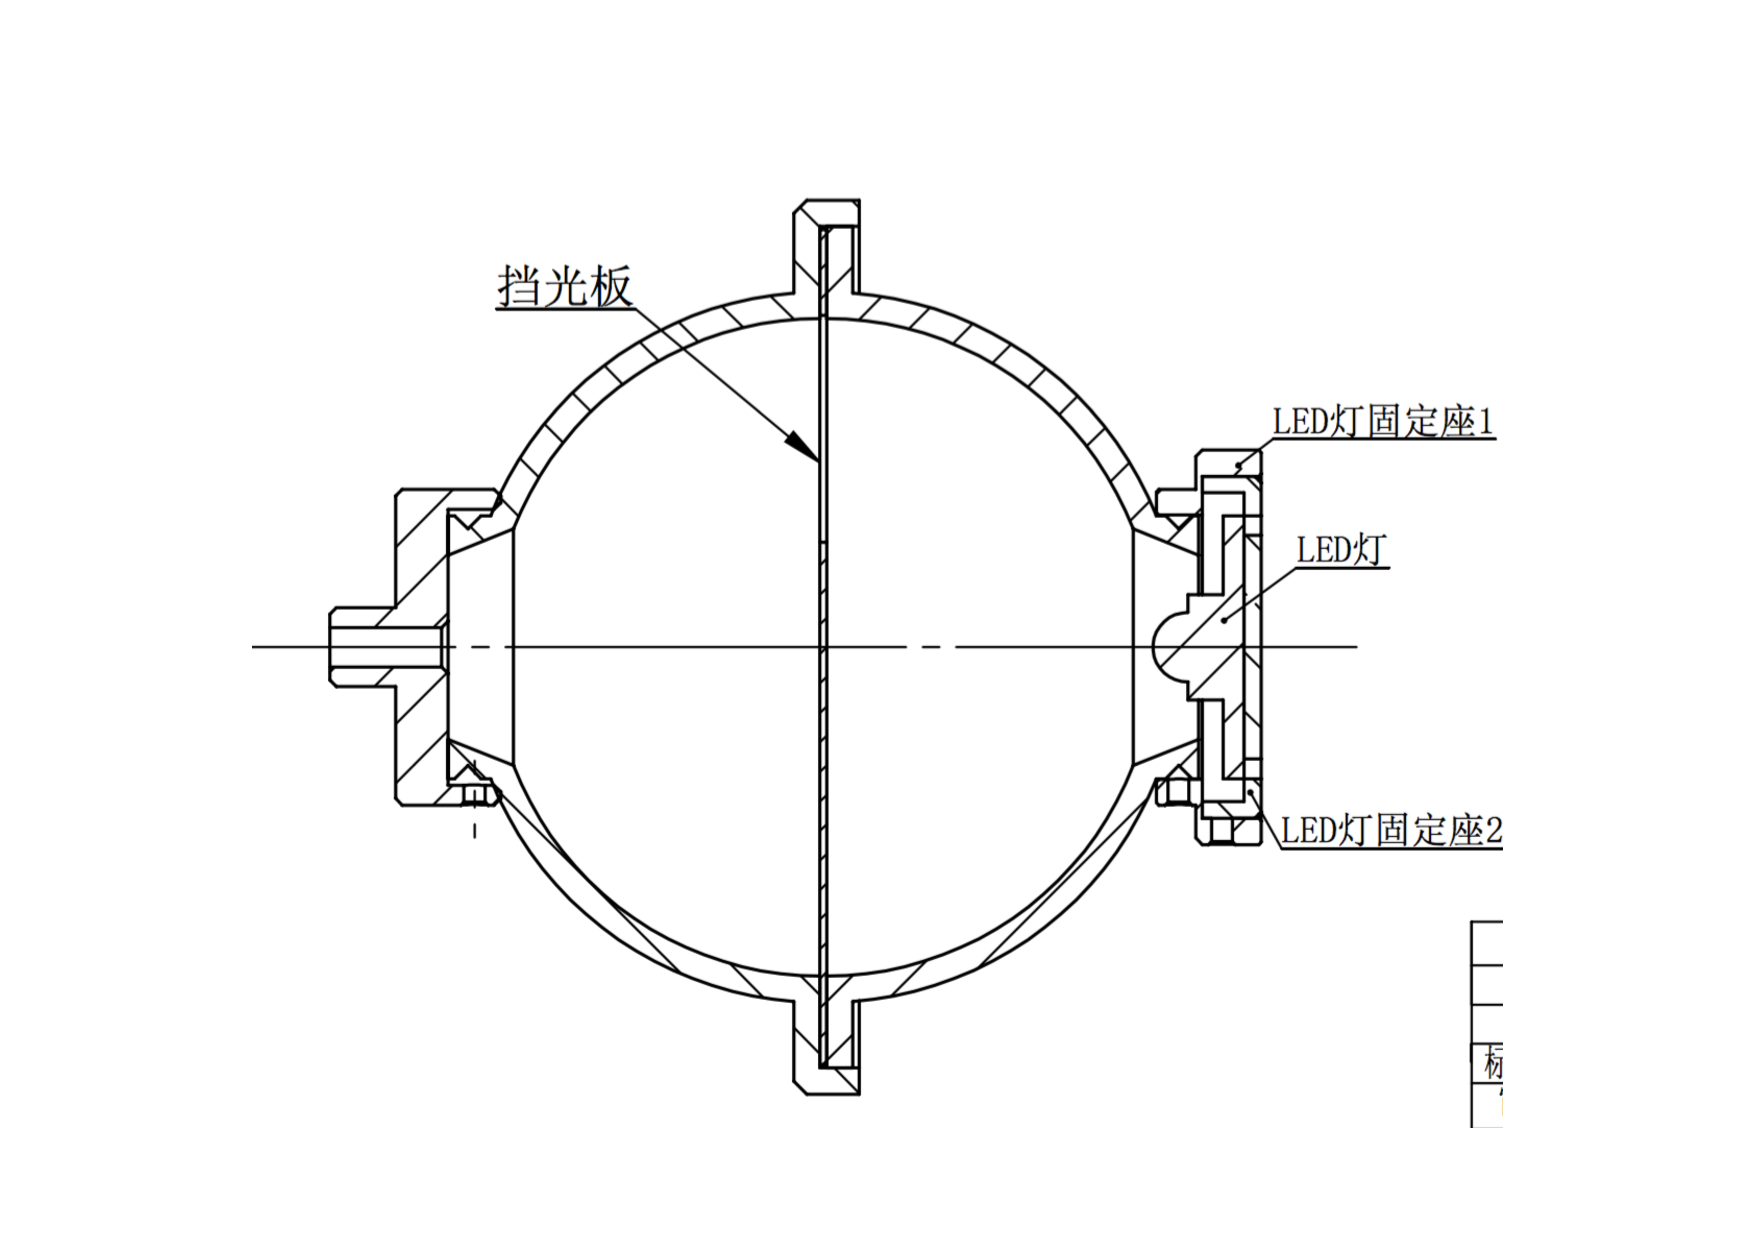
\includegraphics[width=75mm]{is_drawing}
		\caption{Drawing of the 5 cm integrating sphere.}
		\label{fig:is_drawing}
	\end{subfigure}
	\begin{subfigure}[t]{45mm}
		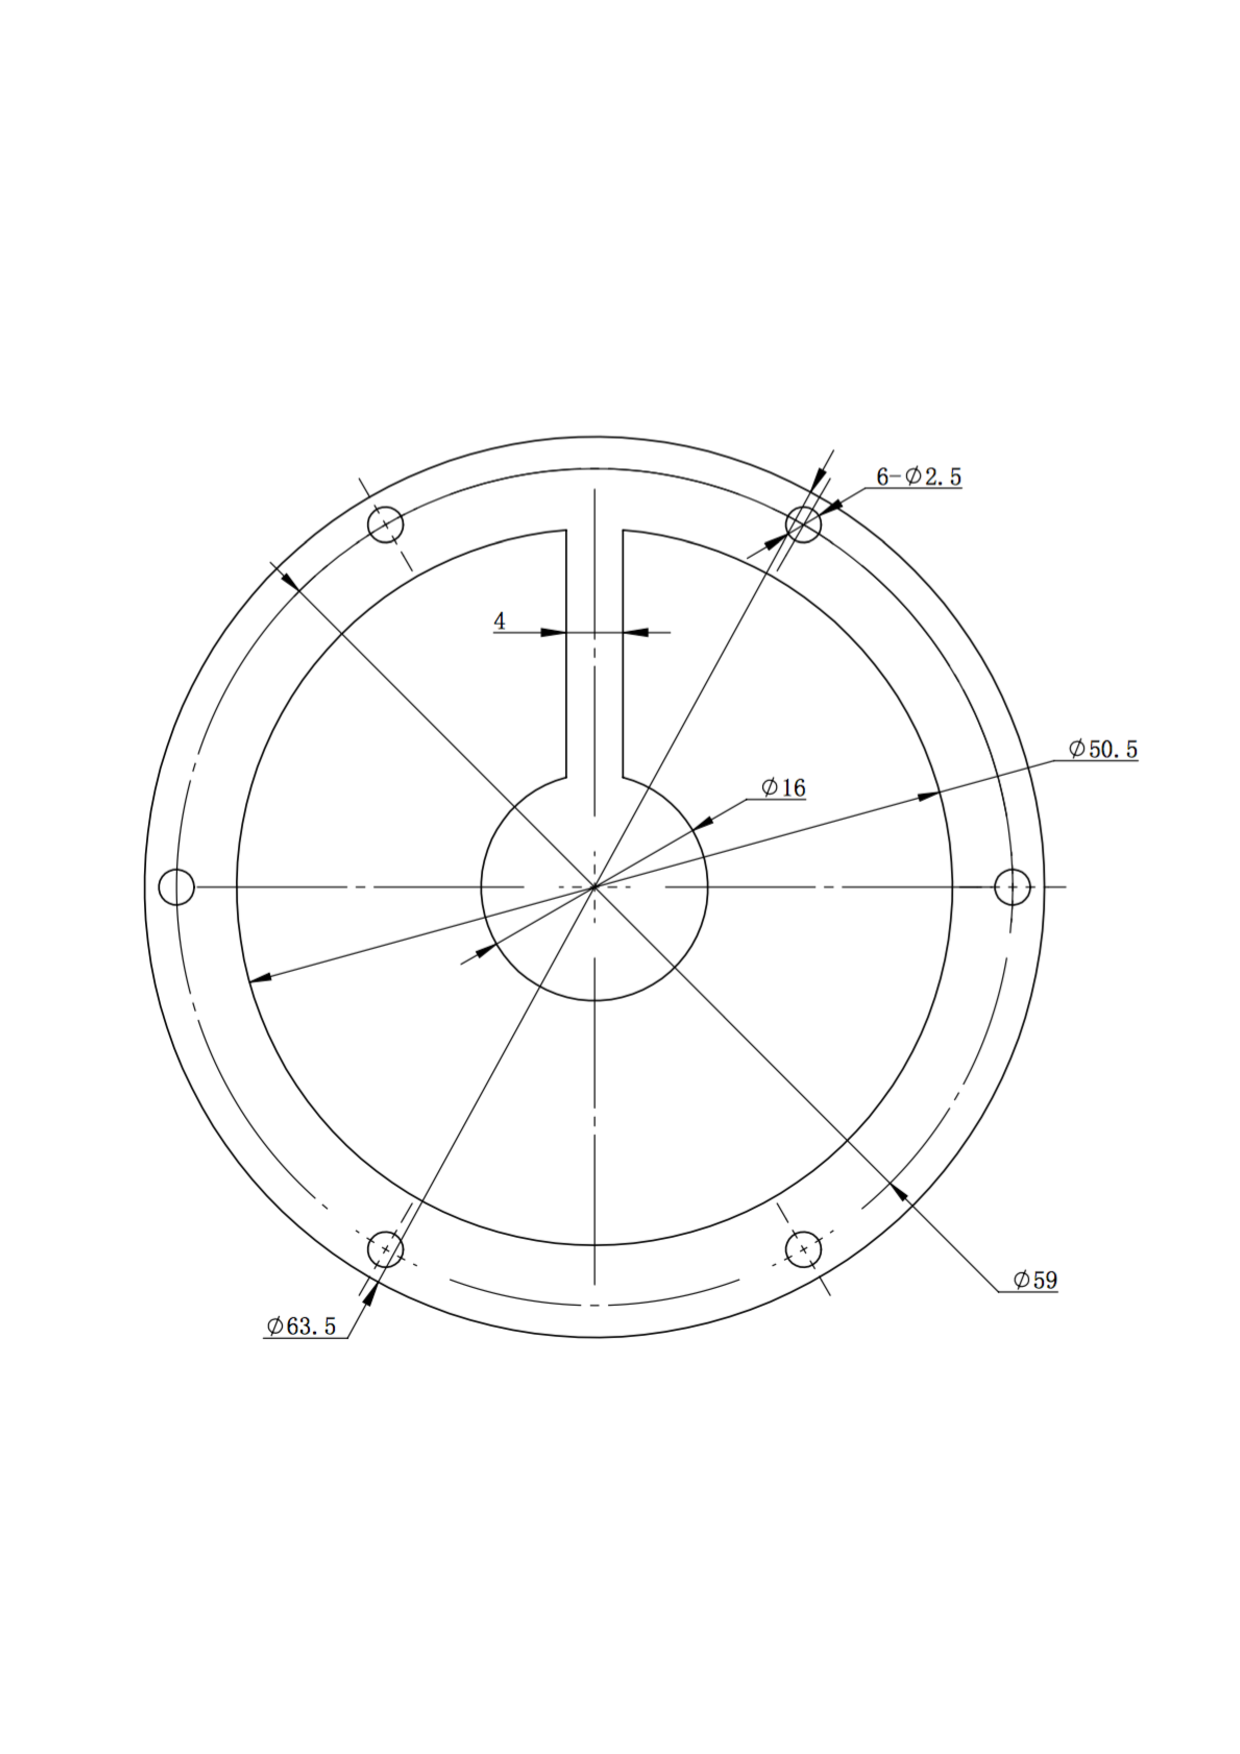
\includegraphics[width=45mm]{baffle}
		\caption{Baffle of the 5 cm integrating sphere.}
		\label{fig:baffle}
	\end{subfigure}
	\caption{Integrating sphere used in the test bench.}
	%\label{fig:FIG2}
\end{figure}

\begin{figure}
\centering
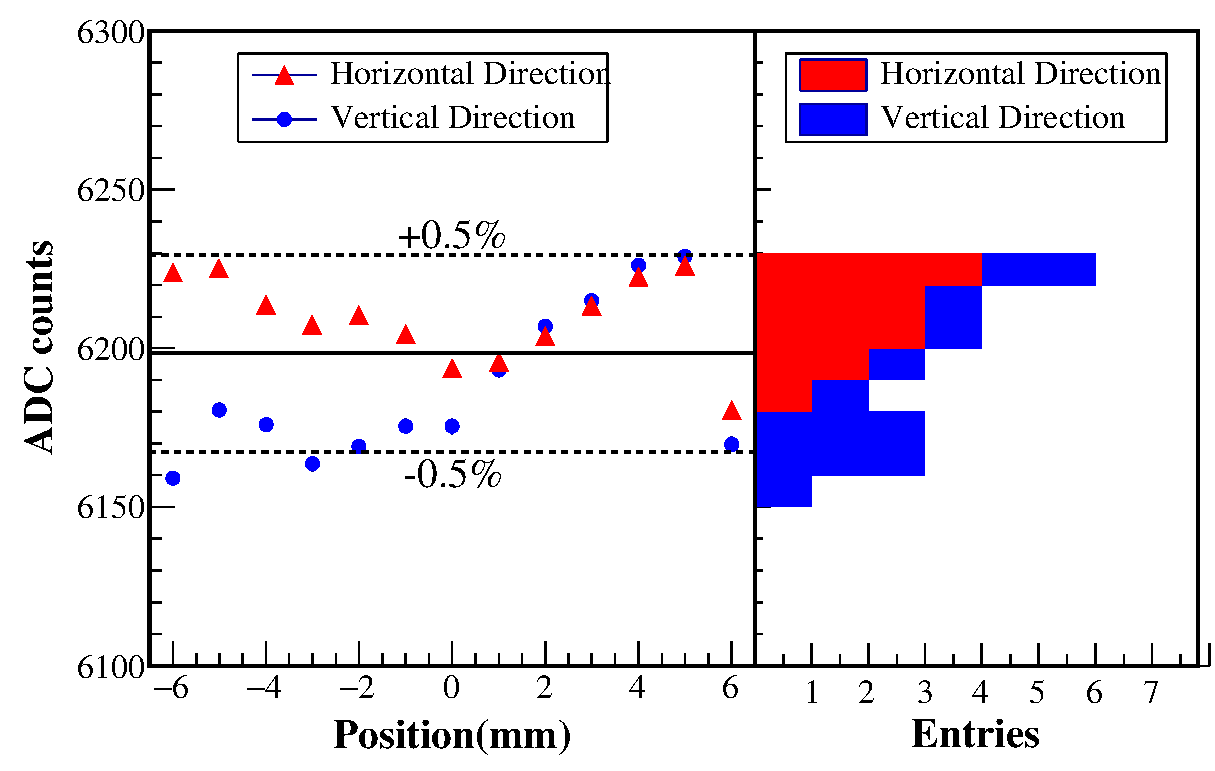
\includegraphics[width=0.7\linewidth]{uniformity_integrationsphere}
\caption{Uniformity of the integrating sphere}
\label{fig:uniformity_integrationsphere}
\end{figure}

\subsection{Question: More infos about R4443}
\textit{Original statements: The paper refers to the Hamamatsu R4443 photomultiplier that however is not listed in the Hamamatsu catalogue and surfing the web I did not find a data sheet for it. If, as I believe to understand, the R4443 is a modified version of the R647 it should be clearly stated and the differences highlighted.}\newline

\textbf{Answer:}\newline
The complete version number of the PMT used in DAMPE-PSD is R4443 Mod2. It is a modified version of R4443 tube, which has been used before in the GLAST-FERMI project.But I'm not sure whether it's a modified version of R647 or not. R4443 Mod2 has been specifically customized for the DAMPE-PSD project, thus it is not listed in the Hamamatsu catalogue. There are two major improvements of R4443 Mod2 against its previous versions, i.e. its structure has been ruggedized for space usage and a low-noise cathode material has been adopted to eliminate the dark current. Table~\ref{tab:r4443} gives the major characteristics of R4443 Mod2. 
\begin{longtabu} to 0.8\linewidth{lX}
	\caption{Major Characteristics of R4443 Mod2\label{tab:r4443}}\\
	\toprule[1.5pt]
	\textbf{Characteristics} & \textbf{Typical Value} \\ 
	\midrule
	\endfirsthead
	
	%\toprule[1.5pt]
	\multicolumn{2}{ c }{continuing Table~\ref{tab:r4443}}\\
	%性能参数 & 典型值 \\ 
	\midrule
	\endhead
	
	%\bottomrule[1.5pt]
	\endfoot
	
	\bottomrule[1.5pt]
	\endlastfoot
	
	Spectrum response & 300$\sim$650 \si{\nano\meter} \\
	Peak of spectrum response  & \SI{375}{\nano\meter} \\
	Photocathode material & low-noise Bialkali \\
	Minimum effective cathode area & \SI{10}{\milli\meter} \\
	Working temperature  & \SI{-30}{\celsius}$\sim$\SI{50}{\celsius} \\
	Rising time  & \SI{2.5}{\nano\second} \\
	Transit time  & \SI{24}{\nano\second} \\
	Dynode number & 10 \\
	Typical gain & \SI{1.0E6}{} \\
	Maximum working voltage & \SI{1250}{\volt}\\
	weight & \SI{11}{\g}\\
	Diameter  & \num[separate-uncertainty]{14.5(7)} \si{\milli\meter} \\
	Typical dark current & \SI{0.5}{\nano\ampere}\\
	Maximum dark current & \SI{4.0}{\nano\ampere} \\
\end{longtabu}

\section{Reviewer 2}
\textit{Original statement: Do the fiber transmission difference have something to do with the bending of fibers?
Will this degree of bending change during a certain characterization?}\newline

\textbf{Answer:}\newline


More explanation about PSD detector mechanism.

\section{Reviewer3}
Original statements:
\begin{enumerate}
	\item Check the references, some mistakes here and there
	\item Summary should be more elaborative
	\item Change the black background of Fig.3(a)
\end{enumerate}
\end{document}
